\documentclass[conference,a4paper]{IEEEtran}
\IEEEoverridecommandlockouts
\usepackage{cite}
\usepackage{amsmath,amssymb,amsfonts}
\usepackage{graphicx}
\usepackage{textcomp}
\usepackage{xcolor}
\usepackage{booktabs}
\usepackage{multirow}
\usepackage{float}
\usepackage{tikz}
\usetikzlibrary{positioning,arrows.meta,calc}
\usepackage{pgfplots}
\pgfplotsset{compat=1.18}
\usepgfplotslibrary{groupplots}

\newcommand{\parhead}[1]{\par\vspace{2pt}\noindent\textbf{#1}\par\nobreak}

\begin{document}

\title{Cross-Variety Initialization and Alignment-Supervised Durations for One-Hour Hakka Speech Synthesis}

\author{\IEEEauthorblockN{Chien-Chih Fang}
\IEEEauthorblockA{\textit{Master Program in Intelligent}\\
\textit{Computing and Big Data}\\
\textit{Chung Yuan Christian University}\\
Taoyuan, Taiwan\\
tom30112@gmail.com}
\and
\IEEEauthorblockN{I Elizabeth Cha\textsuperscript{*}}
\IEEEauthorblockA{\textit{Master Program in Intelligent}\\
\textit{Computing and Big Data}\\
\textit{Chung Yuan Christian University}\\
Taoyuan, Taiwan\\
icha@cycu.edu.tw\\
\textsuperscript{*}Corresponding author}
\and
\IEEEauthorblockN{Shin-Shin Kao}
\IEEEauthorblockA{\textit{Department of Applied Mathematics}\\
\textit{Chung Yuan Christian University}\\
Taoyuan, Taiwan\\
shinshin@cycu.edu.tw}}

\maketitle

\begin{abstract}
Hakka is a tonal language with several regional varieties, many of which have little recorded speech. This paper studies neural text-to-speech (TTS) for two Taiwanese Hakka varieties, Sixian and Hailu, when only one hour of target-variety speech is available. In such models, a duration predictor decides how long each sound lasts, and this timing shapes the rhythm of speech, the realization of tones, and checked syllables, which end in an unreleased stop and typically have a short vowel. With one hour of data, however, the model must learn its alignments, and therefore its duration targets, from very little speech. This paper proposes XAD-TTS, a training recipe for Matcha-TTS that combines cross-variety initialization with forced-alignment duration supervision: the model is initialized from a model of a closely related Hakka variety, and an enlarged duration predictor is trained on forced-alignment durations instead of the model's own alignments. Across three training seeds, XAD-TTS raises the share of checked-syllable vowels whose durations, measured on synthesized waveforms, are within 30\,ms of the corresponding natural-speech durations from 71.0\% to 81.3\% for Sixian and from 69.4\% to 82.2\% for Hailu, close to full-data baselines trained on 48.0 and 47.2 hours of speech on this measure. It also reduces mel-cepstral distortion by 0.33 and 0.24\,dB and improves objective tone classification, and an automatic speech recognition analysis shows better agreement with natural speech for checked-syllable codas and tone marks.
\end{abstract}

\begin{IEEEkeywords}
duration modeling, forced alignment, Hakka, low-resource languages, text-to-speech, transfer learning
\end{IEEEkeywords}

\section{Introduction}

Hakka is a Sinitic tonal language spoken in several regional varieties. In Taiwan, Sixian and Hailu are two major Hakka varieties. They share many consonants and vowels but differ in their tone systems. Although Hakka speech technology has begun to emerge~\cite{chen2024voxhakka}, recorded speech resources remain limited for individual varieties, making it difficult to develop TTS systems when only a small amount of target-variety data is available.

Many recent neural TTS models are non-autoregressive: a duration predictor first decides how many acoustic frames each input symbol receives, and a decoder then generates speech with that fixed timing~\cite{ren2021fastspeech2,mehta2024matcha}. The predicted durations determine the length of the expanded input representation and strongly influence the timing of the synthesized speech. In tonal languages, vowel duration can affect the time available for realizing a pitch contour, which is an important acoustic cue for lexical tone. In Hakka, timing also matters for checked syllables, which end in an unreleased stop, written as \textit{-b}, \textit{-d}, or \textit{-g} in the romanization used in this study. These syllables typically have short vowel nuclei, so vowel duration is one of the cues that distinguish them from other syllables.

Models such as Matcha-TTS~\cite{mehta2024matcha} obtain their duration targets themselves: during training, monotonic alignment search (MAS)~\cite{kim2020glow} aligns input symbols with acoustic frames, and the duration predictor learns to reproduce these alignments. Learning alignments inside the TTS model removes the need for an external aligner~\cite{kim2020glow,badlani2022one}. The alignments are thus estimated by the model being trained, from the same data. With one hour of speech, both the acoustic model and its alignments are learned from little data, and errors in the alignments are passed on to the duration predictor.

For a low-resource Hakka variety, two additional resources can help. First, a closely related variety may have much more recorded speech. Sixian and Hailu share many consonants and vowels, so a model trained on one variety may provide useful initialization for the other, much as pre-training on other data~\cite{chung2019semi} and models of related, better-resourced languages~\cite{chen2019crosslingual,xu2020lrspeech} have been used to reduce the data needed for TTS. Second, a forced aligner such as the Montreal Forced Aligner (MFA)~\cite{mcauliffe2017mfa}, trained on recordings of the variety, provides phone durations that do not depend on the TTS model, as used in FastSpeech~2~\cite{ren2021fastspeech2}. This paper proposes XAD-TTS, short for cross-variety initialization with alignment-supervised durations, which combines the two for Hakka. The target model starts from a model of the other variety, and its duration predictor, enlarged to use a wider context, is trained on aligner durations instead of MAS alignments. The combination is intended to improve duration modeling under limited target-variety training data. The aligner is not required during synthesis; it is also used in this study to measure segment durations during evaluation. Each ingredient has been used separately before; XAD-TTS combines them for a pair of closely related varieties and measures their effect on segment timing. The main contributions are as follows:
\begin{itemize}
\item \textbf{XAD-TTS:} A training recipe for Matcha-TTS that combines cross-variety initialization, alignment-supervised durations, and an enlarged duration predictor, without adding any component at synthesis time.
\item \textbf{Experiments across data sizes:} Evaluation on Sixian and Hailu using three training seeds at 1\,h and 10\,h, together with single-seed full-data baseline references at 48.0\,h and 47.2\,h.
\item \textbf{Evaluation beyond spectral distortion:} In addition to mel-cepstral distortion, segment durations measured on the synthesized waveforms, objective tone classification, and agreement with natural speech in automatic speech recognition (ASR).
\end{itemize}

\section{Method}

\subsection{Baseline model}
The baseline system, denoted Base, uses the original Matcha-TTS architecture~\cite{mehta2024matcha} and is trained from scratch. Matcha-TTS encodes input symbols into per-symbol features and predicts their durations. The features are expanded according to the durations, and a conditional flow-matching decoder~\cite{lipman2023flow} generates a mel spectrogram. A HiFi-GAN vocoder~\cite{kong2020hifigan} then converts the mel spectrogram into a waveform.

During training, MAS estimates the alignment between input symbols and mel frames, and the duration predictor is trained using the resulting durations. The training objective consists of duration, prior, and flow-matching losses. In the original inference procedure, predicted durations are rounded up to whole frames. The rounding rule used in this study is described below.

\subsection{Cross-variety initialization}
The source model is a model of the other Hakka variety, trained from scratch in the same way as Base on all of that variety's training data. A Sixian target model is therefore initialized from a Hailu model trained on 47.2\,h of Hailu speech, and a Hailu target model from a Sixian model trained on 48.0\,h of Sixian speech. Both varieties use one shared symbol table. For target-model initialization, parameters with matching names and shapes are copied from the source model, except for the speaker embeddings and, in XAD-TTS, the enlarged duration predictor. These components are re-initialized, no parameters are frozen, and the optimizer is restarted.

Training data are normalized with statistics calculated from the target-variety training data. Because the copied model buffers contain the mel-normalization statistics of the source variety, synthesis also uses the target-variety statistics.

\subsection{Alignment-supervised durations}
For each variety, an MFA acoustic model was trained on all HAT TTS recordings of that variety and their transcripts, including the validation and test recordings, before the data were split, using a pronunciation lexicon derived from the romanization by deterministic rules. MFA training uses only audio and transcripts, without duration labels, and the same alignments provide the natural reference durations used in the evaluation. Over 99\% of the utterances were successfully aligned; the remaining 42 Sixian and 143 Hailu utterances were excluded from all subsets. The resulting phone intervals are converted into frame counts using a hop size of 256 samples at a sampling rate of 22.05\,kHz, corresponding to approximately 11.6\,ms per frame.

Matcha-TTS inserts blank tokens between input symbols. Silence between two phones is assigned to the pause symbol at that position if the text contains one, and otherwise to the blank token between the two phones. Every symbol, including each blank, receives at least one frame, taken from the preceding symbol when possible. The resulting durations replace MAS-derived durations during training. They serve as targets for the duration loss and determine the feature expansion used in the prior and decoder losses.

\subsection{Larger duration predictor and rounding}
To increase the capacity of the duration predictor, its kernel size is changed from 3 to 5 and its number of channels from 256 to 512. With its two convolution layers, each prediction then depends on nine neighboring input symbols instead of five. When cross-variety initialization is applied in XAD-TTS, the enlarged duration predictor and speaker embeddings are re-initialized.

Rounding every predicted duration up can lengthen the total duration. Each trained model therefore uses either rounding up or cumulative rounding (rounding the running sum, which preserves the total length), chosen on the validation set only: the rule whose rounded vowel-nucleus durations have the smaller mean absolute error with respect to the MFA durations, averaged over checked and other syllables, is selected. The same procedure is applied to all systems, including Base.

XAD-TTS combines cross-variety initialization, alignment-supervised durations, and the enlarged duration predictor; its name refers to cross-variety initialization (X) and alignment-supervised durations (AD). Fig.~\ref{fig:overview} illustrates the training, synthesis, and evaluation procedures. The target model is initialized from the source-variety model and trained on the one-hour target training speech and text, while MFA-derived durations from the same data provide supervision for the enlarged duration predictor and alignment information for training. After training, the model synthesizes speech from test text. The synthesized speech is then evaluated using natural test speech as a reference.

\begin{figure}[H]
\centering
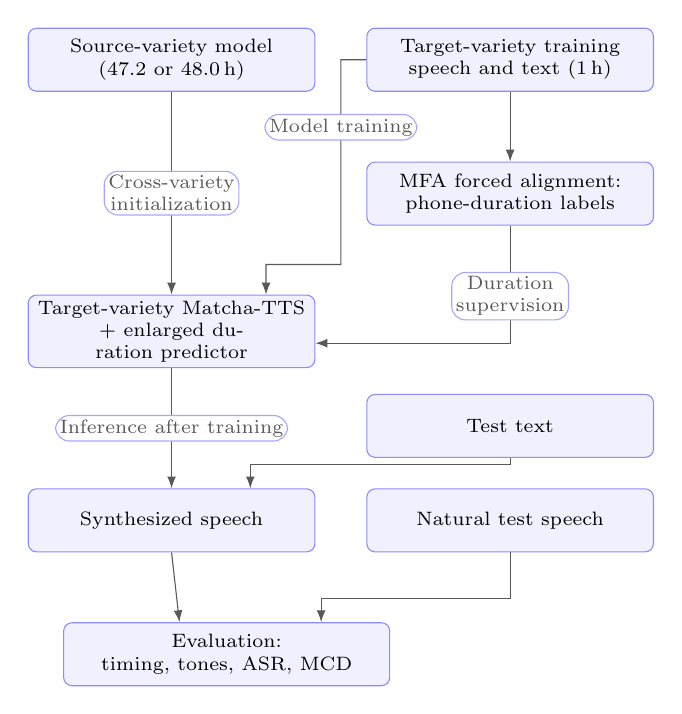
\begin{tikzpicture}[
  font=\scriptsize,
  box/.style={draw=blue!45, rounded corners=3pt, align=center, minimum height=8mm, text width=35mm, inner sep=2pt, fill=blue!6},
  tag/.style={draw=blue!35, rounded corners=5pt, fill=white, font=\scriptsize, inner sep=1.5pt, align=center},
  arr/.style={-{Latex[length=1.5mm]}, gray!70!black}]
\node[box] (src)   at (0, 0) {Source-variety model\\(47.2 or 48.0\,h)};
\node[box] (train) at (4.3, 0) {Target-variety training\\speech and text (1\,h)};
\node[box] (mfa)   at (4.3, -1.7) {MFA forced alignment:\\phone-duration labels};
\node[box] (tts)   at (0, -3.45) {Target-variety Matcha-TTS\\+ enlarged duration predictor};
\node[box] (text)  at (4.3, -4.65) {Test text};
\node[box] (syn)   at (0, -5.85) {Synthesized speech};
\node[box] (nat)   at (4.3, -5.85) {Natural test speech};
\node[box, text width=40mm] (eval) at (0.7, -7.55) {Evaluation:\\timing, tones, ASR, MCD};
\draw[arr] (train) -- (mfa);
\draw[arr] (src) -- node[tag]{Cross-variety\\initialization} (tts);
\draw[arr] (train.west) -- (2.15,0) -- node[tag, pos=0.33]{Model training} (2.15,-2.6) -- (1.2,-2.6) -- ([xshift=12mm]tts.north);
\draw[arr] (mfa.south) |- node[tag, pos=0.3]{Duration\\supervision} ([yshift=-1.5mm]tts.east);
\draw[arr] (tts) -- node[tag]{Inference after training} (syn);
\draw[arr] (text.south) |- ([xshift=10mm, yshift=3mm]syn.north) -- ([xshift=10mm]syn.north);
\draw[arr] (syn.south) -- ([xshift=-6mm]eval.north);
\draw[arr] (nat.south) |- ([xshift=12mm, yshift=3mm]eval.north) -- ([xshift=12mm]eval.north);
\end{tikzpicture}
\caption{Overview of XAD-TTS.}
\label{fig:overview}
\end{figure}

\section{Experimental Setup}

\subsection{Data}
The experiments use the TTS part of the Hakka Across Taiwan (HAT) corpus~\cite{hat2024}: read speech in Sixian and Hailu, each by one professional female and one professional male speaker. Utterances with code-switching or syllable contractions are excluded. Validation and test sets are defined by recording prompt, so their prompts never occur in training of the same variety. Training subsets of 1\,h and 10\,h are balanced across the two speakers and nested (the 10\,h set contains the 1\,h set). Each syllable is split into initial, vowel, and final consonant by fixed rules. In the main experiments, the tone is attached to the vowel, so a vowel with a given tone is one symbol (``joint'' symbols). The first results experiment also tests ``separate'' symbols, in which the tone is a separate input; the two varieties then share 84\% of their symbols instead of 55\%.

\subsection{Systems and training}
Three systems are compared, all with joint symbols: Base, the original Matcha-TTS baseline trained from scratch with MAS durations; +AD, trained from scratch with alignment-supervised durations (AD) only; and XAD, the full XAD-TTS recipe, which adds cross-variety initialization and the enlarged predictor to +AD. Each is trained with Adam (learning rate $10^{-4}$, batch 16) for a fixed 40{,}000 steps with three training seeds (1234, 123, 2026) at 1\,h and 10\,h, and the 40{,}000-step checkpoint is evaluated. As a high-resource reference, Base is also trained on the full pool (48.0\,h of Sixian, 47.2\,h of Hailu) with early stopping and a single seed. One 40{,}000-step run takes about 2\,h on a single RTX~5070~Ti GPU; Base has 20.9\,M parameters and XAD 22.4\,M.
Synthesis uses 10 sampling steps of the flow-matching decoder, temperature 0.667, and the universal HiFi-GAN vocoder.

\subsection{Evaluation}
For each variety, 100 test sentences (50 per speaker) are randomly sampled from the test set and synthesized by every system. The text of 3 Sixian and 10 Hailu sentences also occurs in the training data of the other variety, which the source model may have seen; excluding them changes the checked-syllable gain of XAD over Base by at most 0.2 percentage points and its MCD reduction by at most 0.005\,dB, so all sentences are kept. 95\% confidence intervals (CIs) are obtained by resampling sentences 5{,}000 times; with several seeds, every seed uses the same resampled sentences. Values in square brackets denote these 95\% CIs.

\parhead{Spectral distortion}
Mel-cepstral distortion (MCD)~\cite{kubichek1993mcd} is computed on 24 WORLD~\cite{morise2016world} mel-cepstral coefficients (without $c_0$) after dynamic time warping and averaged over five generation seeds per sentence.

\parhead{Segment timing}
Each synthesized waveform is force-aligned with the same MFA model, and the duration of every vowel nucleus is compared with the same nucleus in the natural recording. Timing accuracy is the share of nuclei within $\pm$30\,ms (2.6 frames) of the natural duration, reported separately for checked and other syllables, together with the Pearson correlation $\rho$ of checked-syllable nucleus durations. At 1\,h, tolerances of $\pm$20 and $\pm$50\,ms give the same ranking of Base, +AD, and XAD.

\parhead{Tone recognition}
A gradient-boosting classifier is trained on up to 3{,}000 natural utterances of the full training pool with acoustic features only: a five-point F0 contour of the nucleus in semitones relative to the speaker median, its mean and slope, log-duration, voicing ratio, and the F0 of neighboring syllables. Its accuracy on the synthesized syllables is reported, and its accuracy on all natural test recordings serves as a reference.

\parhead{Speech recognition check}
The 1B Omnilingual ASR model~\cite{omnilingual2025}, set to Hakka, transcribes Hakka in a romanization with tone diacritics and stop codas \textit{-p}, \textit{-t}, \textit{-k}. Each natural recording and its synthetic versions are transcribed, and the transcripts are aligned word by word. The measures are the character error rate (CER) between the ASR transcript of synthesized speech and that of the corresponding natural recording, computed on Latin letters and tone marks with spaces, digits, and non-Latin characters removed and pooled over sentences, the retention of checked syllables (natural-transcript words ending in \textit{-p}/\textit{-t}/\textit{-k} whose aligned synthetic word still does), the letter-similarity gap between checked and other words, and the tone-mark agreement of aligned words. Twenty of the 200 test sentences (12 Sixian, 8 Hailu) are excluded because the recognizer's output for the natural recording was mostly non-Latin text; the remaining 180 sentences are the same for all systems, and the results are pooled over the two varieties. Copy-synthesis, in which natural mel spectrograms are passed through the same vocoder, serves as a reference condition.

\section{Results}

\subsection{Cross-variety initialization}
In a preliminary sweep over five data sizes from 1 to 48\,h, initialization lowered the validation loss in 16 of 20 settings; the gain was largest at 1\,h (0.08--0.13) and was close to zero under the full-data conditions (48.0 and 47.2\,h), so the analysis focuses on 1\,h. Table~\ref{tab:transfer} compares MCD between training from scratch and cross-variety initialization with 1\,h of target-variety data and one training seed. Each model is trained for 40{,}000 steps with validation every 1{,}000 steps, and the checkpoint with the lowest validation loss is evaluated; this differs from the main experiments, where the 40{,}000-step checkpoint is evaluated. $\Delta$ is the MCD of the initialized model minus that of the model trained from scratch, computed per sentence from unrounded values, so it can differ by 0.01 from the difference of the rounded means. The 95\% CI in brackets is obtained by resampling sentences 10{,}000 times within each speaker. Table~\ref{tab:transfer} uses its own 100 test sentences without these overlapping texts, so its MCD values are not comparable with those of the main experiments.

\begin{table}[H]
\centering
\caption{Effect of Cross-Variety Initialization on MCD.}
\label{tab:transfer}
\footnotesize
\begin{tabular}{llccc}
\toprule
Target & Symbols & Scratch & Init. & $\Delta$ [95\% CI] \\
\midrule
Sixian & joint    & 6.36 & 5.99 & $-$0.36 [$-$0.39, $-$0.34] \\
Sixian & separate & 6.17 & 6.08 & $-$0.09 [$-$0.12, $-$0.06] \\
Hailu  & joint    & 6.46 & 6.59 & +0.13 [+0.09, +0.18] \\
Hailu  & separate & 6.48 & 6.22 & $-$0.26 [$-$0.30, $-$0.22] \\
\bottomrule
\end{tabular}
\end{table}

Initialization lowers MCD in three of four settings, by up to 0.36\,dB, but raises it for Hailu with joint symbols (+0.13\,dB), mostly for the male speaker (+0.35\,dB vs.\ $-$0.08\,dB). Initialization alone is therefore helpful but not uniformly so, and XAD-TTS pairs it with alignment supervision.

\subsection{Main results at one hour}
Table~\ref{tab:main} summarizes the results. Checked and Other are the percentages of checked-syllable and other-syllable vowels whose duration is within $\pm$30\,ms of the natural duration; $\rho$ is the Pearson correlation between synthesized and natural vowel durations of checked syllables; $\Delta$MCD is the MCD difference from Base (1\,h), where negative values are better; and Tone is the accuracy of the tone classifier. The 1\,h system results are averaged over three training seeds. The full-data Base systems, Base (48.0\,h) and Base (47.2\,h), use one training seed, while the natural-recording rows report the classifier accuracy on real speech.

\begin{table}[H]
\centering
\caption{Results for the 1\,h Systems and Full-Data References.}
\label{tab:main}
\footnotesize
\setlength{\tabcolsep}{3.6pt}
\begin{tabular}{lccccc}
\toprule
System & Checked & Other & $\rho$ & $\Delta$MCD & Tone \\
 & (\%) $\uparrow$ & (\%) $\uparrow$ & $\uparrow$ & (dB) $\downarrow$ & (\%) $\uparrow$ \\
\midrule
\multicolumn{6}{l}{\textit{Sixian}} \\
Base (1\,h)       & 71.0 & 63.7 & 0.535 & ---            & 64.3 \\
+AD (1\,h)        & 77.0 & 70.4 & 0.651 & $-$0.12        & 69.0 \\
XAD (1\,h)        & \textbf{81.3} & \textbf{74.0} & \textbf{0.738} & \textbf{$-$0.33} & \textbf{73.0} \\
Base (48.0\,h)    & 81.1 & 73.9 & 0.767 & ---            & ---  \\
Natural recordings & ---  & ---  & ---   & ---            & 71.5 \\
\midrule
\multicolumn{6}{l}{\textit{Hailu}} \\
Base (1\,h)       & 69.4 & 54.9 & 0.576 & ---            & 62.1 \\
+AD (1\,h)        & 77.7 & 58.9 & 0.676 & $-$0.10        & 64.2 \\
XAD (1\,h)        & \textbf{82.2} & \textbf{65.9} & \textbf{0.743} & \textbf{$-$0.24} & \textbf{67.3} \\
Base (47.2\,h)    & 83.0 & 68.6 & 0.797 & ---            & ---  \\
Natural recordings & ---  & ---  & ---   & ---            & 67.1 \\
\bottomrule
\end{tabular}
\end{table}

Both +AD and XAD improve the measured duration accuracy over Base, and XAD provides further gains over +AD under the evaluated settings. Alignment supervision alone (+AD) raises the share of checked-syllable vowels within $\pm$30\,ms by 6.0 (Sixian) and 8.3 (Hailu) percentage points. XAD adds another 4.3 and 4.5 points, reaching 81.3\% [77.6, 85.2] and 82.2\% [78.0, 86.4] against 71.0\% [66.9, 75.2] and 69.4\% [65.3, 73.8] for Base, which is close to the high-resource references (81.1\% and 83.0\%) for this measure. Other syllables improve as well (63.7\% to 74.0\% and 54.9\% to 65.9\%), and the correlation of checked-syllable durations rises from 0.54 to 0.74 (Sixian) and from 0.58 to 0.74 (Hailu), still below the references (0.77 and 0.80). XAD lowers MCD by 0.33 [0.31, 0.35] and 0.24 [0.20, 0.28]\,dB, two to three times the reduction from +AD (0.12 and 0.10\,dB), and the XAD reduction is observed for all three seeds. Tone-classification accuracy rises by 8.8 [7.7, 9.9] and 5.3 [4.4, 6.2] percentage points and XAD exceeds +AD by 4.1 and 3.2 percentage points. These paired differences are pooled over seeds and syllables and can differ by 0.1 from the rounded means in Table~\ref{tab:main}. The classifier accuracy on XAD-generated speech is close to that on natural recordings (measured on all test sentences). This does not imply that the synthesized tones are more natural or more accurate than human speech.

\subsection{Effect of data size}
Fig.~\ref{fig:size} compares checked-syllable duration accuracy at 1\,h and 10\,h of target-variety training data, with three training seeds per system. The full-data Base references use one training seed. For the 1\,h systems and the full-data references, the 95\% CIs span about $\pm$4 percentage points.

\begin{figure}[H]
\centering
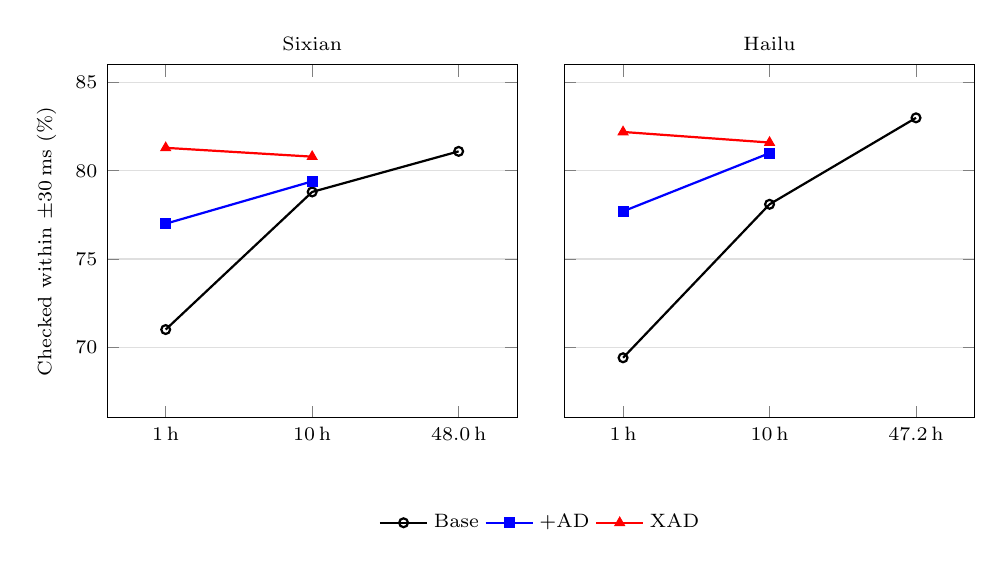
\begin{tikzpicture}
\begin{groupplot}[
  group style={group size=2 by 1, horizontal sep=6mm, y descriptions at=edge left},
  width=0.56\columnwidth, height=0.5\columnwidth,
  xtick=data, enlarge x limits=0.2,
  ymin=66, ymax=86, ytick={70,75,80,85}, ymajorgrids, grid style={gray!25},
  tick label style={font=\scriptsize}, label style={font=\scriptsize}, title style={font=\scriptsize, yshift=-1.5mm},
  legend style={font=\scriptsize, draw=none, fill=none, legend columns=3, at={(1.06,-0.24)}, anchor=north},
  every axis plot/.append style={thick, mark size=1.6pt}]
\nextgroupplot[title=Sixian, symbolic x coords={1\,h,10\,h,48.0\,h}, ylabel={Checked within $\pm$30\,ms (\%)}]
\addplot[black, mark=o] coordinates {(1\,h,71.0) (10\,h,78.8) (48.0\,h,81.1)};
\addplot[blue, mark=square*] coordinates {(1\,h,77.0) (10\,h,79.4)};
\addplot[red, mark=triangle*] coordinates {(1\,h,81.3) (10\,h,80.8)};
\legend{Base, +AD, XAD}
\nextgroupplot[title=Hailu, symbolic x coords={1\,h,10\,h,47.2\,h}]
\addplot[black, mark=o] coordinates {(1\,h,69.4) (10\,h,78.1) (47.2\,h,83.0)};
\addplot[blue, mark=square*] coordinates {(1\,h,77.7) (10\,h,81.0)};
\addplot[red, mark=triangle*] coordinates {(1\,h,82.2) (10\,h,81.6)};
\end{groupplot}
\end{tikzpicture}
\caption{Checked-syllable duration accuracy across data sizes.}
\label{fig:size}
\end{figure}

The gains over Base are smaller at 10\,h than at 1\,h. At 10\,h, XAD improves checked-syllable duration accuracy by 2.0 percentage points for Sixian and 3.5 percentage points for Hailu. It also reduces MCD by 0.24\,dB and 0.16\,dB, respectively, whereas +AD has MCD differences of +0.04\,dB and +0.03\,dB relative to Base. At 1\,h, XAD achieves duration accuracy close to the full-data Base references on the $\pm$30\,ms measure; XAD additionally uses the source-variety model, so this comparison does not imply that only one hour of Hakka speech is involved.

\subsection{Speech recognition check}
Table~\ref{tab:asr} presents ASR-based results pooled across the two varieties using 180 test sentences. The measures include CER between the synthetic-speech and natural-speech ASR transcripts, checked-coda retention, the letter-similarity gap (Gap) between checked and other words, and tone-mark agreement. Copy-synthesis is included as a reference condition.

\begin{table}[H]
\centering
\caption{ASR-Based Evaluation Results.}
\label{tab:asr}
\footnotesize
\setlength{\tabcolsep}{3.2pt}
\begin{tabular}{lcccc}
\toprule
System & CER & Checked & Gap & Tone \\
 & (\%) $\downarrow$ & kept (\%) $\uparrow$ & $\uparrow$ & marks (\%) $\uparrow$ \\
\midrule
Base (1\,h)          & 22.2 & 77.8 & $-$4.1 & 73.9 \\
+AD (1\,h)           & 21.8 & 81.5 & $-$1.5 & 76.7 \\
XAD (1\,h)           & 21.7 & \textbf{82.6} & \textbf{$-$0.5} & 77.1 \\
Base (47.2/48.0\,h)  & 19.6 & 80.1 & $-$3.7 & 77.2 \\
\midrule
Copy-synthesis       & 9.8  & 89.4 & +0.2 & 88.9 \\
\bottomrule
\end{tabular}
\end{table}

The ASR analysis provides an additional evaluation that does not directly use the MFA timing measurements or the tone classifier. Relative to Base, XAD changes CER by $-$0.5 percentage points with a 95\% CI of [$-$2.7, +1.9], so the observed difference does not establish a clear CER improvement; the full-data Base reference has a lower CER ($-$2.6 [$-$4.5, $-$0.5]). The ASR transcripts retain checked codas more often (+4.8 percentage points [1.6, 8.0]), the checked-word similarity gap narrows from $-$4.1 to $-$0.5 (+3.6 [1.2, 6.0]), and tone-mark agreement increases by 3.2 percentage points [1.9, 4.4]. +AD alone already narrows the gap (+2.6 [0.4, 4.9]), whereas the full-data Base reference does not (+0.4 [$-$2.0, 2.9]) despite a similar tone-mark gain; this suggests that alignment-supervised durations, rather than the amount of target data alone, are associated with the checked-word improvement. XAD substantially reduces the checked-word similarity gap in this ASR-based analysis. A gap remains between XAD and the copy-synthesis reference in ASR transcript agreement (CER 21.7\% vs.\ 9.8\%); the factors contributing to this gap require further investigation.

\subsection{Negative results}
Several additions to XAD were compared directly with XAD: inference-time scaling of vowel durations (three seeds), a higher dropout rate in the duration predictor, pre-training of the duration predictor on source-variety durations, replay of source-variety data during target training (one training seed each), and averaging the predicted durations of the three seeds. None of them provided consistent improvements over XAD under the evaluated settings.

\section{Discussion and Limitations}
At 1\,h of target-variety training data, +AD improves checked-syllable duration accuracy over Base (6.0 of the 10.3 percentage-point gain for Sixian and 8.3 of 12.8 for Hailu), and XAD provides further gains in the evaluated metrics. Because XAD changes both initialization and predictor capacity, the individual contributions of these two components remain to be isolated.

Several limitations should be considered. The aligner was trained on all recordings of each variety, including the validation and test recordings, and therefore uses more target-variety speech than the one-hour TTS training subset. Because MFA is used for both duration supervision and timing evaluation, alignment errors may affect both stages, although all systems, including Base, are measured with the same aligner. In addition, the full-data Base reference uses one training seed, and in Table~\ref{tab:transfer} the best validation checkpoint of every initialized model occurred at the first or second validation point (1{,}000 or 2{,}000 steps), so a finer validation interval might change these values. The ASR model and tone classifier are imperfect evaluation tools; on natural speech, the classifier reaches 71.5\% accuracy for Sixian and 67.1\% for Hailu.

\section{Conclusion}
XAD-TTS combines cross-variety initialization, alignment-supervised durations, and an enlarged duration predictor. With 1\,h of target-variety training speech, XAD-TTS improves checked-syllable duration accuracy, MCD, and objective tone-classification accuracy for both Sixian and Hailu. On the $\pm$30\,ms duration measure, its results are close to those of the full-data Base references. An additional ASR-based analysis shows improved agreement for checked-syllable codas and tone marks relative to the natural-speech transcripts.
The aligner is not required during synthesis. A 40{,}000-step target-model training run takes approximately two hours on a single RTX~5070~Ti GPU; this time excludes source-model training, forced alignment, and data preparation. Future work includes listening tests and further experiments to examine the contribution of individual system components.

\section*{Acknowledgment}
The research was funded by the National Science and Technology Council of the Republic of China under contract number NSTC114-2115-M-033-004. HAT was provided by the Hakka Affairs Council/ACLCLP (No.~2024-005). No new recordings or identifiable data were collected, and no conflicts have been declared. The GenAI tool was used to assist with English translation, improve readability, and refine English grammar. After using the tool, the authors reviewed and edited the content as needed and took responsibility for the final technical content.

% Generated by IEEEtran.bst, version: 1.14 (2015/08/26)
\begin{thebibliography}{10}
\providecommand{\url}[1]{#1}
\csname url@samestyle\endcsname
\providecommand{\newblock}{\relax}
\providecommand{\bibinfo}[2]{#2}
\providecommand{\BIBentrySTDinterwordspacing}{\spaceskip=0pt\relax}
\providecommand{\BIBentryALTinterwordstretchfactor}{4}
\providecommand{\BIBentryALTinterwordspacing}{\spaceskip=\fontdimen2\font plus
\BIBentryALTinterwordstretchfactor\fontdimen3\font minus
  \fontdimen4\font\relax}
\providecommand{\BIBforeignlanguage}[2]{{%
\expandafter\ifx\csname l@#1\endcsname\relax
\typeout{** WARNING: IEEEtran.bst: No hyphenation pattern has been}%
\typeout{** loaded for the language `#1'. Using the pattern for}%
\typeout{** the default language instead.}%
\else
\language=\csname l@#1\endcsname
\fi
#2}}
\providecommand{\BIBdecl}{\relax}
\BIBdecl

\bibitem{chen2024voxhakka}
L.-W. Chen, H.-S. Lee, and C.-C. Chang, ``{VoxHakka}: A dialectally diverse
  multi-speaker text-to-speech system for {Taiwanese Hakka},''
  arXiv:2409.01548, 2024.

\bibitem{ren2021fastspeech2}
Y.~Ren, C.~Hu, X.~Tan, T.~Qin, S.~Zhao, Z.~Zhao, and T.-Y. Liu, ``{FastSpeech
  2}: Fast and high-quality end-to-end text to speech,'' in \emph{Proc. Int.
  Conf. Learning Representations (ICLR)}, 2021.

\bibitem{mehta2024matcha}
S.~Mehta, R.~Tu, J.~Beskow, {\'E}.~Sz{\'e}kely, and G.~E. Henter,
  ``{Matcha-TTS}: A fast {TTS} architecture with conditional flow matching,''
  in \emph{Proc. IEEE Int. Conf. Acoust., Speech, Signal Process. (ICASSP)},
  2024.

\bibitem{kim2020glow}
J.~Kim, S.~Kim, J.~Kong, and S.~Yoon, ``{Glow-TTS}: A generative flow for
  text-to-speech via monotonic alignment search,'' in \emph{Advances in Neural
  Information Processing Systems (NeurIPS)}, 2020.

\bibitem{badlani2022one}
R.~Badlani, A.~{\L}a{\'n}cucki, K.~J. Shih, R.~Valle, W.~Ping, and
  B.~Catanzaro, ``One {TTS} alignment to rule them all,'' in \emph{Proc. IEEE
  Int. Conf. Acoust., Speech, Signal Process. (ICASSP)}, 2022.

\bibitem{chung2019semi}
Y.-A. Chung, Y.~Wang, W.-N. Hsu, Y.~Zhang, and R.~J. Skerry-Ryan,
  ``Semi-supervised training for improving data efficiency in end-to-end speech
  synthesis,'' in \emph{Proc. IEEE Int. Conf. Acoust., Speech, Signal Process.
  (ICASSP)}, 2019.

\bibitem{chen2019crosslingual}
Y.-J. Chen, T.~Tu, C.~chieh Yeh, and H.~yi~Lee, ``End-to-end text-to-speech for
  low-resource languages by cross-lingual transfer learning,'' in \emph{Proc.
  Interspeech}, 2019.

\bibitem{xu2020lrspeech}
J.~Xu, X.~Tan, Y.~Ren, T.~Qin, J.~Li, S.~Zhao, and T.-Y. Liu, ``{LRSpeech}:
  Extremely low-resource speech synthesis and recognition,'' in \emph{Proc. ACM
  SIGKDD Int. Conf. Knowledge Discovery \& Data Mining (KDD)}, 2020.

\bibitem{mcauliffe2017mfa}
M.~McAuliffe, M.~Socolof, S.~Mihuc, M.~Wagner, and M.~Sonderegger, ``{Montreal
  Forced Aligner}: Trainable text-speech alignment using {Kaldi},'' in
  \emph{Proc. Interspeech}, 2017.

\bibitem{lipman2023flow}
Y.~Lipman, R.~T.~Q. Chen, H.~Ben-Hamu, M.~Nickel, and M.~Le, ``Flow matching
  for generative modeling,'' in \emph{Proc. Int. Conf. Learning Representations
  (ICLR)}, 2023.

\bibitem{kong2020hifigan}
J.~Kong, J.~Kim, and J.~Bae, ``{HiFi-GAN}: Generative adversarial networks for
  efficient and high fidelity speech synthesis,'' in \emph{Advances in Neural
  Information Processing Systems (NeurIPS)}, 2020.

\bibitem{hat2024}
{Hakka Affairs Council}, ``Hakka across {Taiwan} ({HAT}) speech corpus,''
  Distributed by the Association for Computational Linguistics and Chinese
  Language Processing (ACLCLP), catalog no.~2024-005, 2024.

\bibitem{kubichek1993mcd}
R.~F. Kubichek, ``Mel-cepstral distance measure for objective speech quality
  assessment,'' in \emph{Proc. IEEE Pacific Rim Conf. Communications, Computers
  and Signal Processing}, 1993.

\bibitem{morise2016world}
M.~Morise, F.~Yokomori, and K.~Ozawa, ``{WORLD}: A vocoder-based high-quality
  speech synthesis system for real-time applications,'' \emph{IEICE Trans. Inf.
  \& Syst.}, vol. E99-D, no.~7, pp. 1877--1884, 2016.

\bibitem{omnilingual2025}
{Omnilingual ASR team}, ``Omnilingual {ASR}: Open-source multilingual speech
  recognition for 1600+ languages,'' arXiv:2511.09690, 2025.

\end{thebibliography}


\end{document}
